\section{Anomalous Sea Ice Extent correlations}
We are interested in more complex patterns and relations than the seasonal patterns seen in the section above. As such, we ran the same calculations as before on the anomalies for each time series we have. This was done by removing the mean value for every month from each individual value for that month over the dataset, essentially removing the seasonal component of our data. The results here are presented in the same order as the previous section, starting with 2m temperature.
% As described in the results section, we can calculate the anomaly in our data in multiple ways. For the following results we find the anomaly by removing monthly means from each location, essentially removing the interanual seasonal effect and looking at the more unrelated but perhaps more spatially complex structures in the remaining signal.
% \begin{figure}[H]
%     \begin{subfigure}[b]{\textwidth}
%          \centering
%          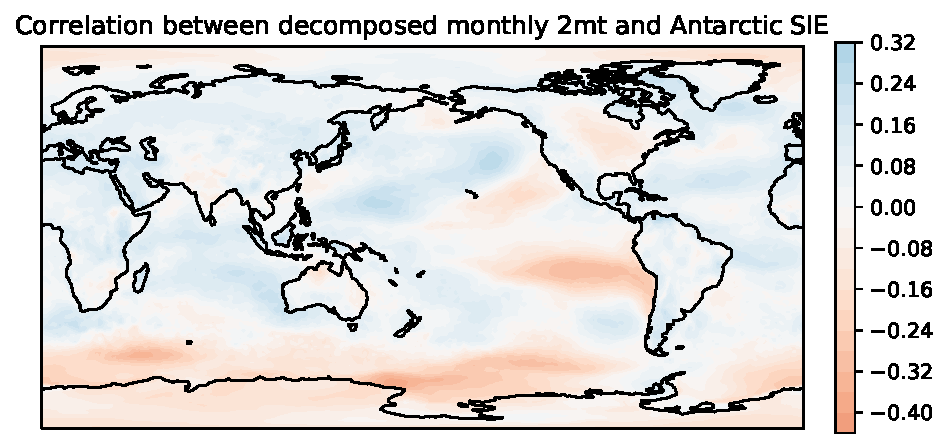
\includegraphics[width=\textwidth]{Images/global_correlation_decomposed_m2mt_sie.pdf}
%         %  \caption{Monthly decomposed 2mt correlated with antarctic SIE}
%          \label{fig:monthly_decomposed_2mt_sie}
%      \end{subfigure}
%      \begin{subfigure}[b]{\textwidth}
%          \centering
%          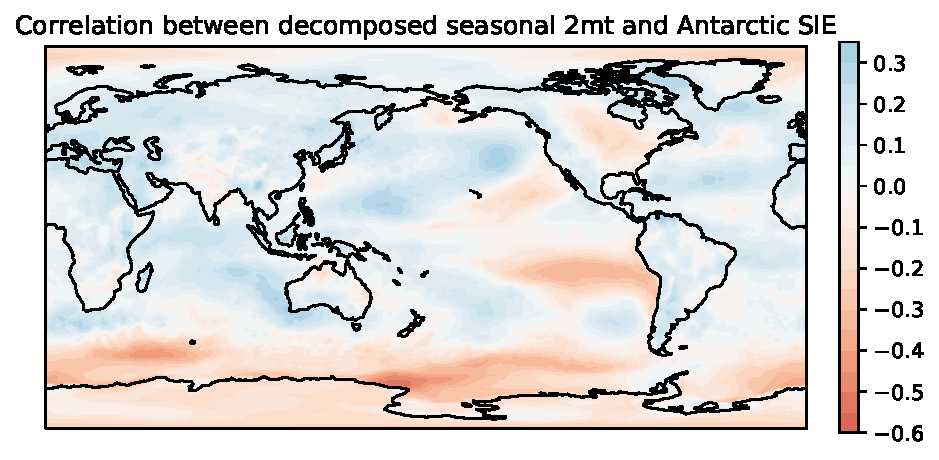
\includegraphics[width=\textwidth]{Images/global_correlation_decomposed_s2mt_sie.pdf}
%         %  \caption{Seasonal decomposed 2mt correlated with antarctic SIE}
%          \label{fig:seasonally_decomposed_2mt_sie}
%      \end{subfigure}
%     \caption{Monthly and seasonal decomposed 2mt correlated with antarctic SIE}
% \end{figure}
% We find little difference between the monthly and seasonal datasets at this point. This is good.
% Additionally, we note that the correlations are low here. This makes sense as there should be no seasonality in the data. Consequently there is also less spatial organisation in the results. The pattern vaguely reminds me of ENSO, so perhaps that is something we could look at moving forward.


\begin{figure}[H]
    \centering
    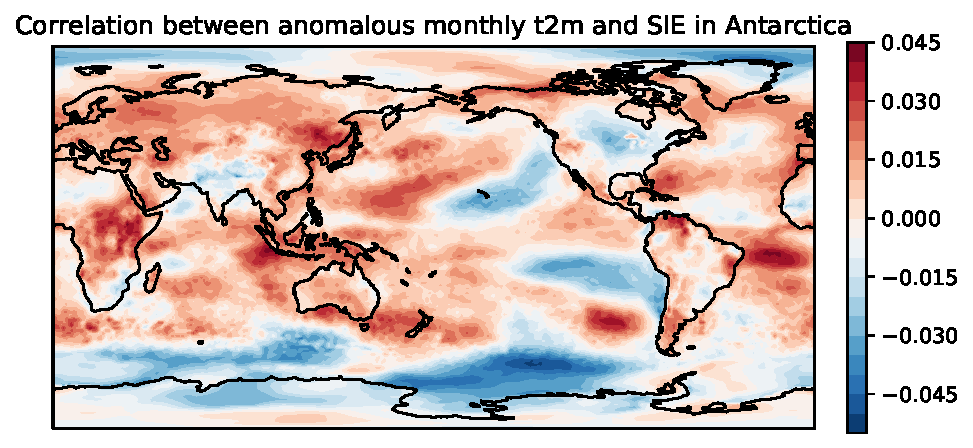
\includegraphics[width=\textwidth]{Images/global_correlation_anomalous_monthly_t2m_sie.pdf}
    \caption{Correlation between anomalous 2m temperature globally and total Sea Ice Extent in Antarctica.}
    \label{fig:t2m_anomalous_sie_corr}
\end{figure}

There is a lot to discuss about this figure, however the thing that stands out the most to me is the IPO pattern. This is something we will potentially want to look at further down the line in our calculations. Next we did the same calculation for surface pressure.

\begin{figure}[H]
    \centering
    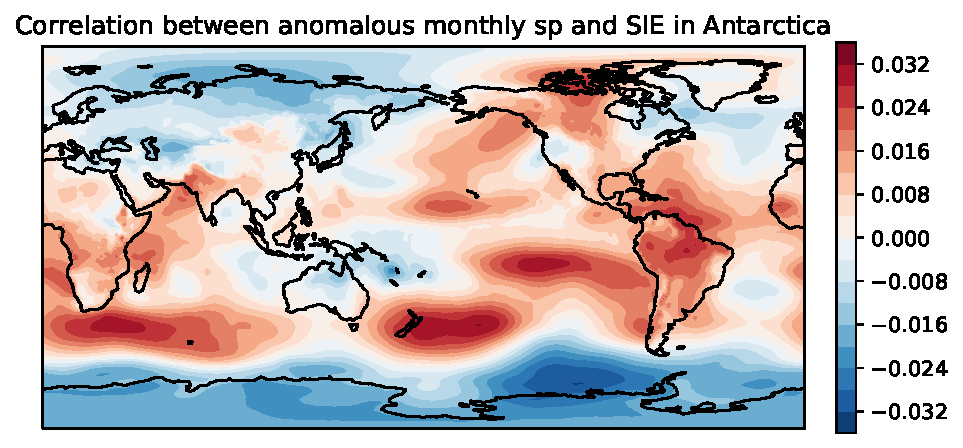
\includegraphics[width=\textwidth]{Images/global_correlation_anomalous_monthly_sp_sie.pdf}
    \caption{Correlation between anomalous surface pressure globally and total Sea Ice Extent in Antarctica.}
    \label{fig:sp_anomalous_sie_corr}
\end{figure}
The first thing to note is how large the signals are for this plot spatially. This is possibly due to how the reanalysis was done or could be showing us something deeper about our climate. I am not entirely sure at this point. Below are the results for the wind correlations.

\begin{figure}[H]
    \centering
    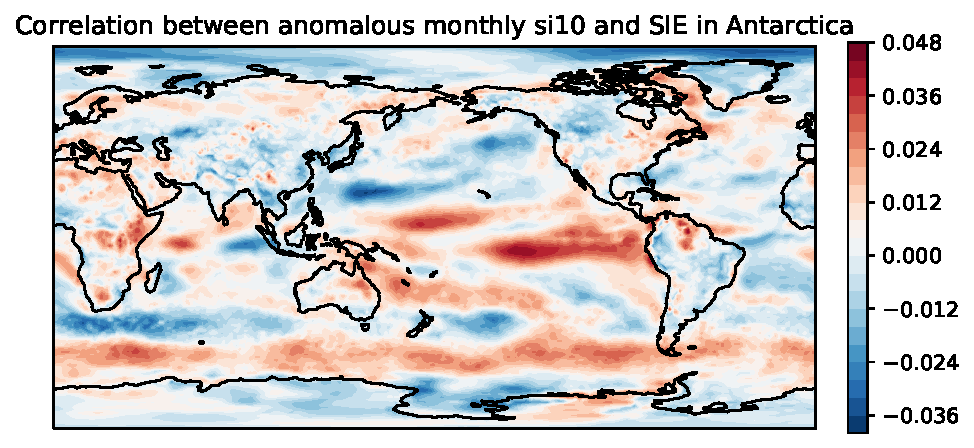
\includegraphics[width=\textwidth]{Images/global_correlation_anomalous_monthly_si10_sie.pdf}
    \caption{Correlation between anomalous 10m wind speed globally and total Sea Ice Extent in Antarctica.}
    \label{fig:si10_anomalous_sie_corr}
\end{figure}

For the total wind speed, the signal which stands out the most looks remarkably like ENSO, this is something we will want to look at further as we continue our analysis.

\begin{figure}[H]
    \centering
    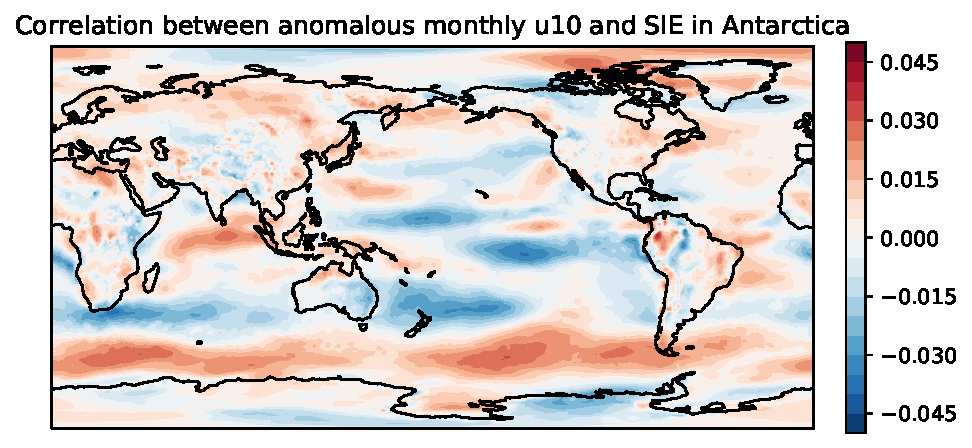
\includegraphics[width=\textwidth]{Images/global_correlation_anomalous_monthly_u10_sie.pdf}
    \caption{Correlation between anomalous u component 10m wind speed globally and total Sea Ice Extent in Antarctica.}
    \label{fig:u10_anomalous_sie_corr}
\end{figure}

For the u component wind, the signal we see could be related to ENSO but it is weaker and less spatially coherent so we cannot be totally sure.

\begin{figure}[H]
    \centering
    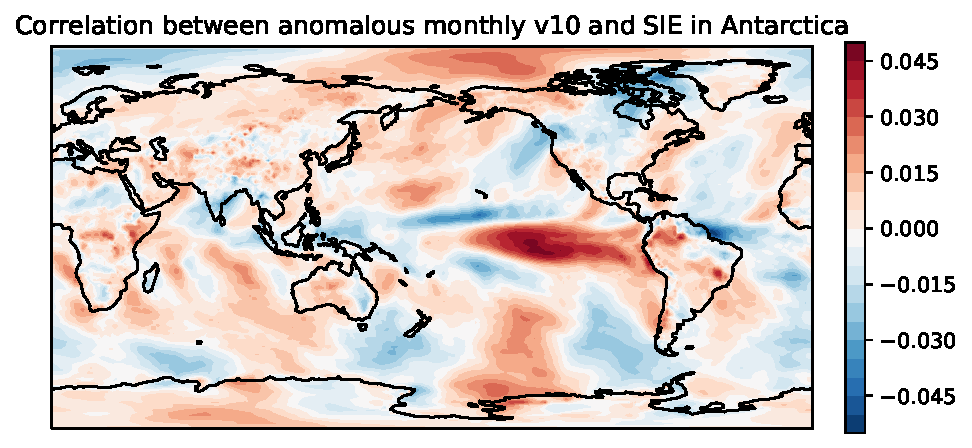
\includegraphics[width=\textwidth]{Images/global_correlation_anomalous_monthly_v10_sie.pdf}
    \caption{Correlation between anomalous v component 10m wind speed globally and total Sea Ice Extent in Antarctica.}
    \label{fig:v10_anomalous_sie_corr}
\end{figure}

For the v component of the wind we see a signal which looks remarkably like ENSO, this is something to look into further.